\documentclass{article}
\title{Study on Term Structure of Interest Rate}
\author{Keiyoo So 5311043}
\date{\today. Mathematic Department,Nihon University}
\usepackage{amsmath}
\usepackage{amssymb}
\usepackage{graphics}
\usepackage{mathrsfs}
\usepackage{setspace}
\usepackage{Sweave}
\begin{document}
\fontsize{10pt}{9pt}
\input{Graduation_Paper-concordance}
\maketitle
\begin{spacing}{1.5}
\begin{abstract}
In this paper I attempt to apply Nelson-Siegel model to study the term structure of Interest by using the dataset of treasury bills of Japan, Unite States and Europe. Then depending on the results of these experiments the yield curve in the three markets, to explain the benefits of Nelson-Siegel model compared to some other models same for the term structure of interest rates.
\\

Keyword: Term Structure\qquad Yield Curve\qquad NS Model\qquad PCA\qquad Times Series  
\end{abstract}
\\
\section{Introduction}
\subsection{Term Structure of Interest Rate}
   Economics theory suggests that one important factor explaining the differences in the interest rates on different securities may be differences in their terms. The relationship between the terms of securities and their market rates of interest rates is called as the term structure of interest rates on securities of a particular type at a particular point in time, economic uses a diagram called a yield curve. As a result, term structure theory is often described as the theory of the yield curve. A way to well understand the term structure of interest rate is parametric models, like \textit{Nelson-Siegel model} by \textit{Nelson} and \textit{Siegel (1987)} and its extension Nelson-Siegel-Svensson model by Svensson (1994); Hull-White model by John Hull and Alan White,etc. All of these models, depend on economic theories, were divided into two factions, \textbf{Equilibrium model} and \textbf{No-Arbitrage model}. Alternative approach uses linear combinations of basis functions, defined over the entire term to maturity spectrum, to fit the discount function. This is referred to as a function-based construction of the yield curve.\\  
  
  So this concept\textemdash the term structure of interest rate was first described in interest rate theories, \textit{Pure Expectation Theory}  by  I.Fischer in 1896, \textit{Liquidity Premium Theory}, \textit{Market Segmentation Theory}, and \textit{Preferred Habituated Theory}. So it is possible to formulate several parametric models based on these theories, that apply specifically to real interest rates. On the other hand, unfortunately, since we cannot observe inflation expectations, so we cannot measure real interest rates directly in the real world.

\subsection{Which model for term structure of interest rates should we use?}
Much of the work done in this area describes models which one we could use, rather than, which one we should use. When we consider which model should we use, then we should know, for sure, a good model must have these properties:
\begin{itemize}
\item[a] simple enough that one can compute answers in reasonable time
\item[b] flexible enough to cover most situations arising in practice
\item[c] well specified, in that required inputs can be easily observed or estimated
\end{itemize}

One fact is that Nelson-Siegel model and Nelson-Siegel-Svensson model both are " be widely used" models by most countries'central bank. Of course both of them have their typical advantages and disadvantages. Nelson-Siegel model is simple and stable for the evaluation, it is quite flexible and very well suited for assessing yields for more bonds and for the time series of returns. Second quite used model is Nelson-Siegel-Svensson model. It provides sufficient  precision adjustment. However, the model has a number of weaknesses, such as limited ability to adapt irregular shapes of the yield curve, the tendency of taking extreme values at the bottom of the curve and a relatively strong dependence on the estimations in different or even nonadjacent segments of the yield curve (Marciniak, 2006).

\subsection{Nelson-Siegel Model}
Nelson-Siegel (1985) suggested forward rate to be estimated as:
\\

\begin{equation}
f(m_i,\mbox{\boldmath $\beta$})=\beta_0 +\beta_1 \exp(-\frac{m_i}{\lambda}) +\beta_2 [(\frac{m_i}{\lambda})\exp(-\frac{m_i}{\lambda})]
\end{equation}\\
\mbox{\boldmath $\beta$}=($\beta_0$,$\beta_1$,$\beta_2$,$\lambda$)\\

The spot rate is the average of instantaneous forward rates
\begin{equation}
s(m_i,\mbox{\boldmath $\beta$})=\frac{1}{m_i} \int_0^{m_i}  f(t,\mbox{\boldmath $\beta$}) \, dt
\end{equation}
resulting in
\begin{equation}
s(m_i,\mbox{\boldmath $\beta$})=\beta_0 + \beta_1 \frac{1-exp(-\frac{m_i}{\lambda})}{\frac{m_i}{\lambda}} + \beta_2 [\frac{1-exp(-\frac{m_i}{\lambda})}{\frac{m_i}{\lambda}}-exp(-\frac{m_i}{\lambda})]
\end{equation}

where,
$m_i$ denotes maturity
\begin{itemize}
\item\ $\beta_0$:Level of Yield Curve
\item\ $\beta_1$:Slope of Yield Curve    
\item\ $\beta_2$:Curvature of Yield Curve
\end{itemize}\\ are parameters that needs to be estimated.
\subsection{Factor Duration}
Given $CF_i$ as cash flow at time $i$, $PV_i$(present value at time $i$)$= \frac {CF_i}{(1+s(m_i))^{m_i}}$, then the price of bond can be calculated by
\begin{equation*}
\begin{split}
   P &=\sum_{i=1}^n PV_i \\
   &= \sum_{i=1}^n \frac{CF_i}{(1+s(m_i))^{m_i}}
\end{split}
\end{equation*}
then we have
\begin{equation*}
\begin{split}
D_{level} &=-\frac{1}{P} \frac{\partial P}{\partial \beta_0}\\
        &=\frac{1}{P} \sum_{i=1}^n m_i \frac{PV_i}{1+s(m_i)}
\end{split}\\
\begin{split}
D_{slope} &=\frac{1}{P} \sum_{i=1}^n m_iA \frac{PV_i}{1+s(m_i)}
\end{split}\\
\begin{split}
D_{curve} &=\frac{1}{P} \sum_{i=1}^n m_iB \frac{PV_i}{1+s(m_i)}
\end{split}
\end{equation*}
where
\begin{equation*}
\begin{split}
A&:\frac{1-exp(-\frac{m_i}{\lambda})}{\frac{m_i}{\lambda}}\\
B&:\frac{1-exp(-\frac{m_i}{\lambda})}{\frac{m_i}{\lambda}}-exp(-\frac{m_i}{\lambda})
\end{split}
\end{equation*}
 And also as we can see from the formula (3) above,\\

$\displaystyle\lim_{m\to \infty}$ s(m,\mbox{\boldmath $\beta$})=$\beta_0$\qquad 
$\displaystyle\lim_{m\to 0}$ s(m,\mbox{\boldmath $\beta$})=$\beta_0$ + $\beta_1$ \\

 Therefore, $\beta_0$ depicts the long term component of interest rate,and the short term component of interest rate is given by $\beta_0$$+$$\beta_1$ as ${m_i\to \infty}$.
 Most researches of term structure of interest rate based on Nelson-Siegel model actually estimate the yield to maturity or the bonds price by analyzing the static samples of interest rate, or by developing a estimated regression equation for the values of independent variables. But on the other hand, it is clear that more than just a common level factor is operative. In the real world, term structure data\textemdash and, correspondingly, modern empirical term structure models\textemdash involve multiple factors.
  From these models, determination of yield uses only maturity. Diebold suggested that yield in each country is actually very different depending on the state of economic factors

\section{Data Description}
 Here I have several datasets of treasury bonds yield to maturity from Bank of Japan and Federal Reserve Bank, both of them were selected with same range that from 2004 to 2013. And a dataset of yield curve from European Central Bank with range from DEC.2006 to JUL.2009.








\begin{center}
\begin{figure}[htbp]
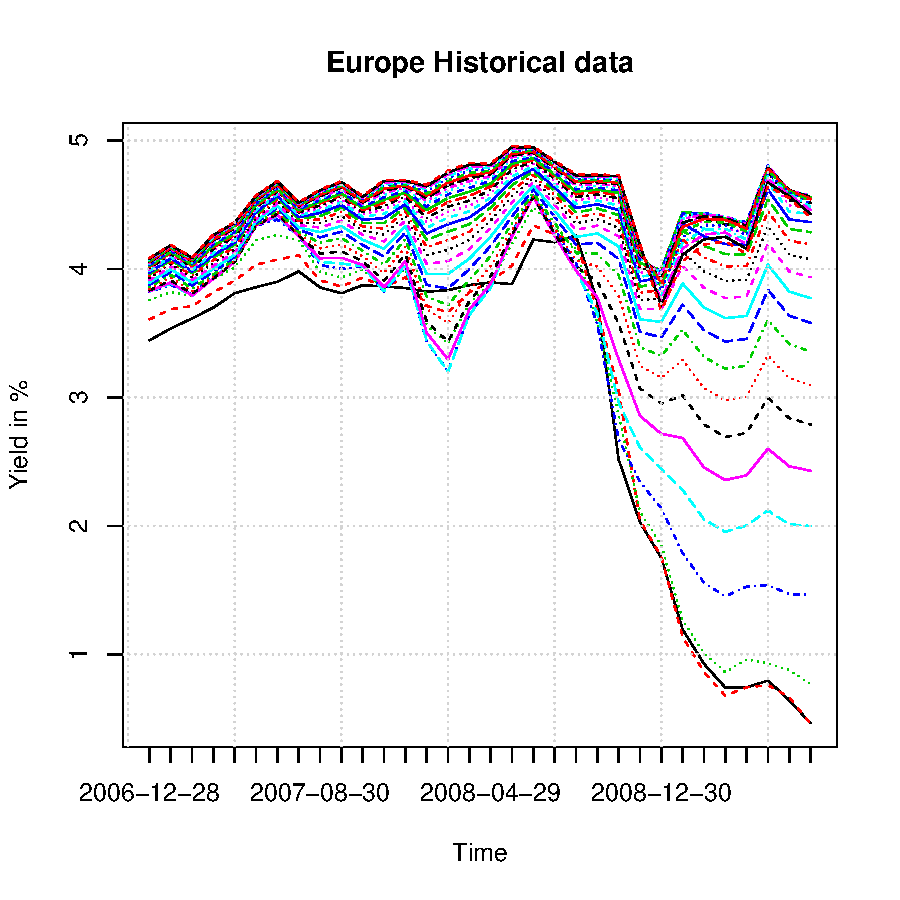
\includegraphics{Graduation_Paper-007}
\end{figure}
\end{center}

\begin{center}
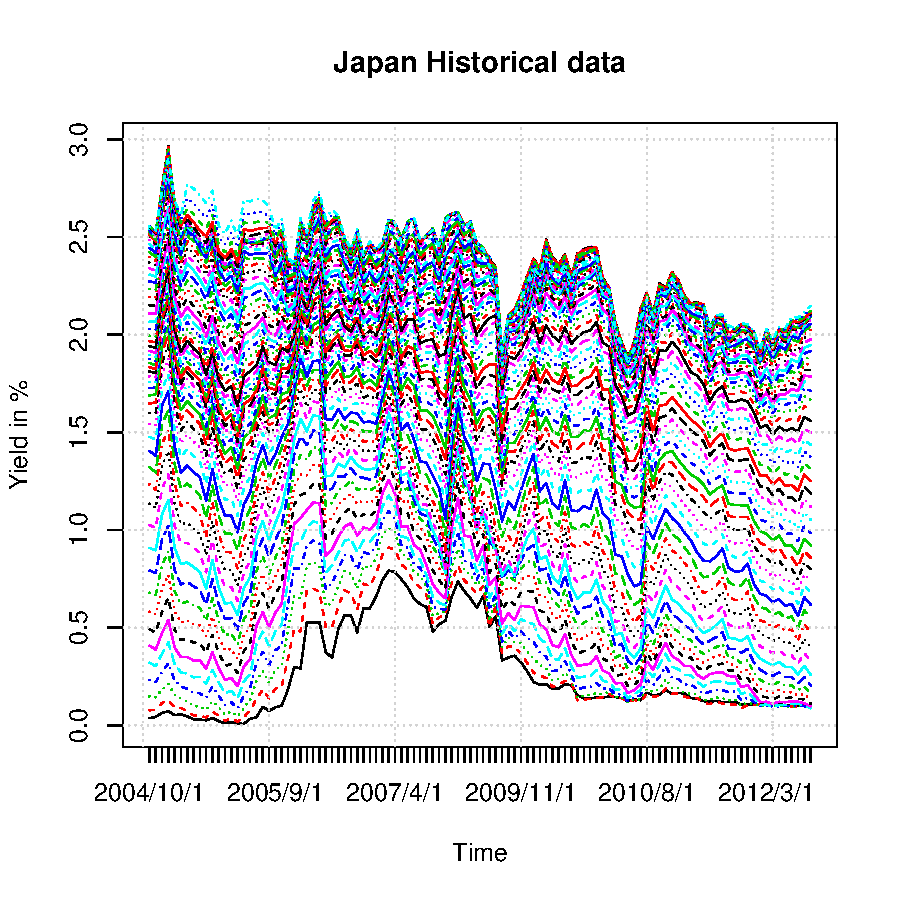
\includegraphics{Graduation_Paper-008}
\end{center}

\begin{center}
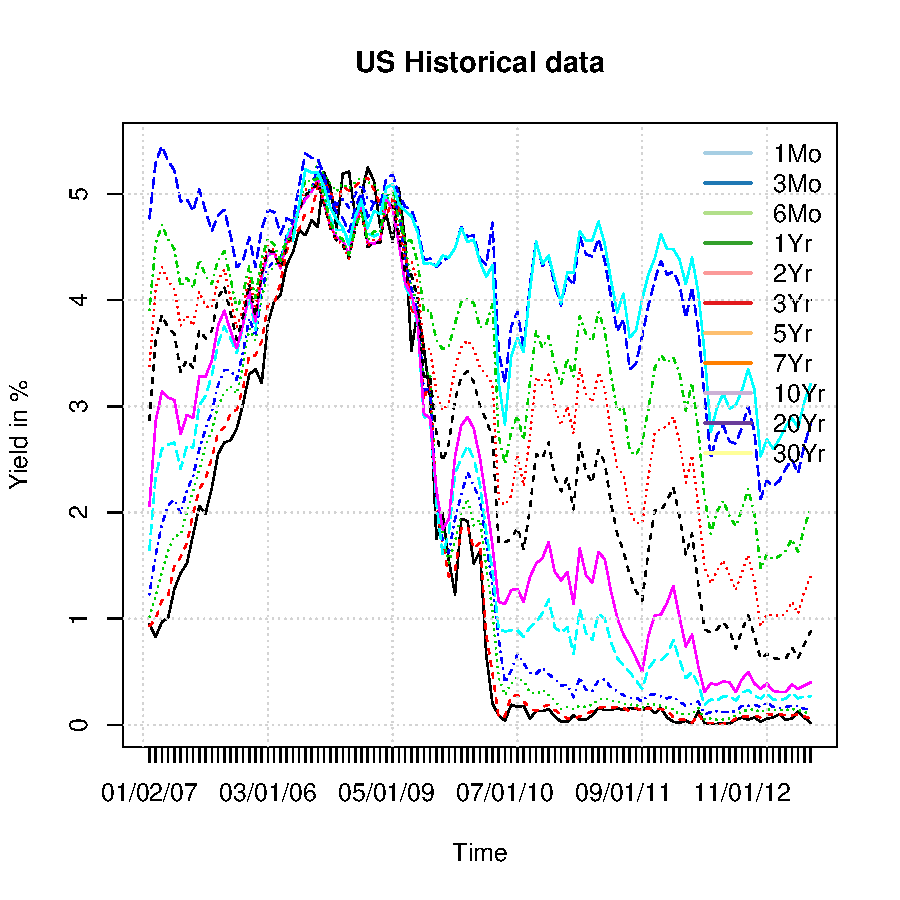
\includegraphics{Graduation_Paper-009}
\end{center}


 As we can see, it is obvious in the plots of ECB yield curve and FRB yield curve that all of the bond yields dropped sharply in a few months during 2007-2008, this phenomenon is one of most impacts of bankruptcy of Lehman Brothers. On the other hand, the overall change in the plot of Japan yield curve is not as sharp as the change of Europe and America looks. One fact is that when the yield of interest rate rises, the price of government bonds drops.
\section{Estimation for parameters}
 Now by using the package "termstrc" in R, I can easily get the estimated parameters of Nelson-Siegel model.
 \subsection{Result of US}
\begin{Schunk}
\begin{Soutput}
---------------------------------------------------
Estimated Nelson/Siegel parameters:
---------------------------------------------------

Number of oberservations: 107 

[[1]]
     beta_0          beta_1            beta_2              tau_1      
 Min.   :3.147   Min.   :-5.4321   Min.   :-6.145064   Min.   :0.200  
 1st Qu.:4.515   1st Qu.:-4.7039   1st Qu.:-4.368298   1st Qu.:1.409  
 Median :4.984   Median :-3.5997   Median :-2.513629   Median :2.013  
 Mean   :4.804   Mean   :-3.1725   Mean   :-2.135497   Mean   :2.046  
 3rd Qu.:5.168   3rd Qu.:-1.3211   3rd Qu.: 0.001124   3rd Qu.:2.808  
 Max.   :5.974   Max.   :-0.3325   Max.   : 1.495122   Max.   :5.994  
\end{Soutput}
\end{Schunk}

\begin{center}
\begin{tabular}{|l||c|}\hline
                        & Goodness of fit \\ \hline
RMSE-yields (in \%)     & 0.1513377   \\ \hline
AABSE-yields (in \%)    & 0.0830996   \\ \hline
\end{tabular}
\end{center}


\begin{itemize}
\item\ {\it AABSE}$_{yield}$ (Average Absolute Mean Error) = $\sum_{i=1}^N$ $\sqrt{\frac{(e_{i,yield}-\bar{e}_{yield})^2}{n}}$
\item\ {\it RMSE}$_{yield}$(Root Mean Squared Error) = $\sqrt{\frac{1}{n}\sum_{i=1}^n (e_i-\bar{e_i})^2}$
\end{itemize}

\begin{center}
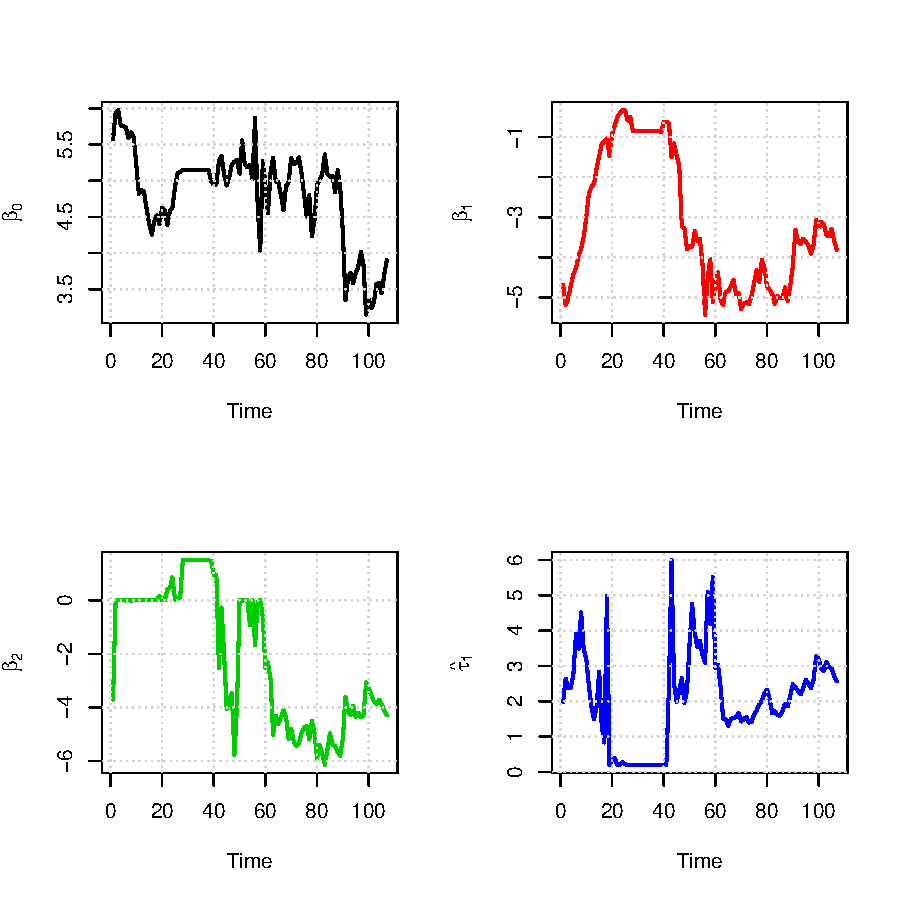
\includegraphics{Graduation_Paper-011}
\end{center}

\begin{center}
\begin{figure}[htbp]
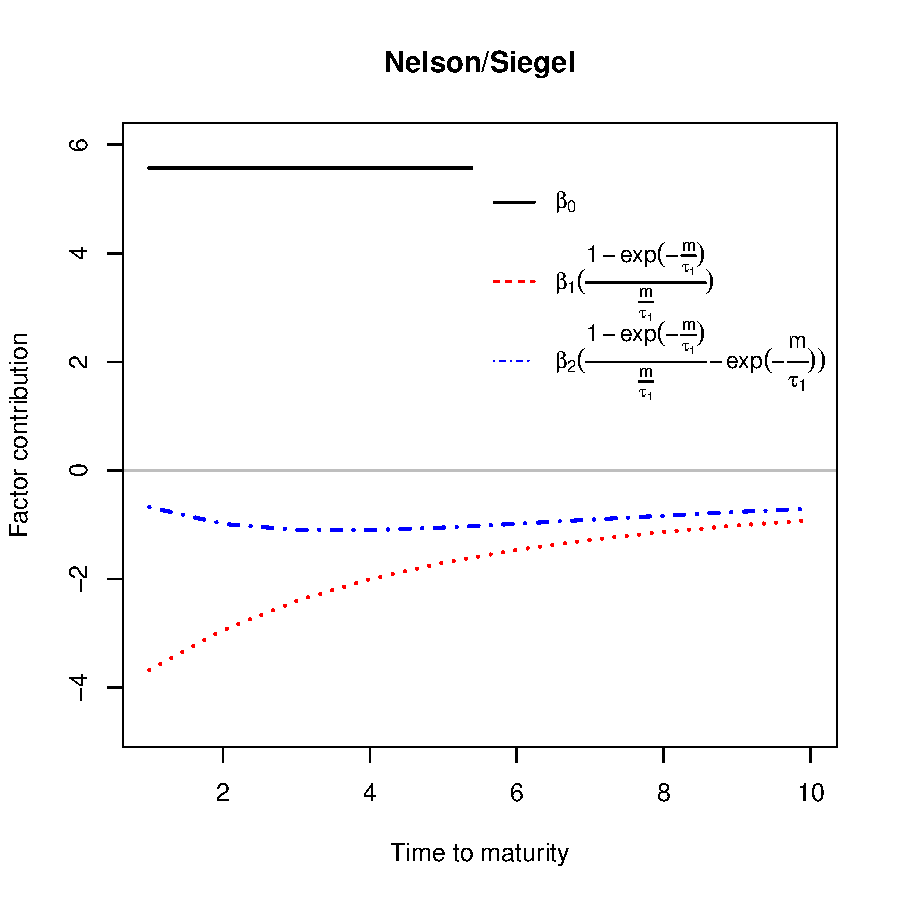
\includegraphics{Graduation_Paper-012}
\caption{Factor contribution, US data}
\end{figure}
\end{center}
 As we already know that Nelson-Siegel model is one of widely used model in practice for fitting the term structure of interest rates. Due to the ease in linearizing the model, a grid search or an OLS approach using a fixed shape parameter are popular estimation procedures. However, the estimated parameters have been reported, by $\mathit{e.g}$ Fabozzi(2005), to behave erratically over time.

\subsection{Result of Japan}
\begin{Schunk}
\begin{Soutput}
---------------------------------------------------
Estimated Nelson/Siegel parameters:
---------------------------------------------------

Number of oberservations: 106 

[[1]]
     beta_0          beta_1           beta_2              tau_1      
 Min.   :2.410   Min.   :-3.534   Min.   :-5.487302   Min.   :2.110  
 1st Qu.:2.898   1st Qu.:-2.876   1st Qu.:-4.720547   1st Qu.:2.580  
 Median :3.061   Median :-2.614   Median :-3.456781   Median :2.794  
 Mean   :3.050   Mean   :-2.656   Mean   :-3.360085   Mean   :3.312  
 3rd Qu.:3.289   3rd Qu.:-2.349   3rd Qu.:-2.876544   3rd Qu.:3.785  
 Max.   :3.644   Max.   :-1.868   Max.   : 0.002765   Max.   :6.000  
\end{Soutput}
\end{Schunk}

\begin{center}
\begin{tabular}{|l||c|}\hline
                        & Goodness of fit \\ \hline
RMSE-yields (in \%)     & 0.0885204   \\ \hline
AABSE-yields (in \%)    & 0.0553115   \\ \hline
\end{tabular}
\end{center}

\begin{center}
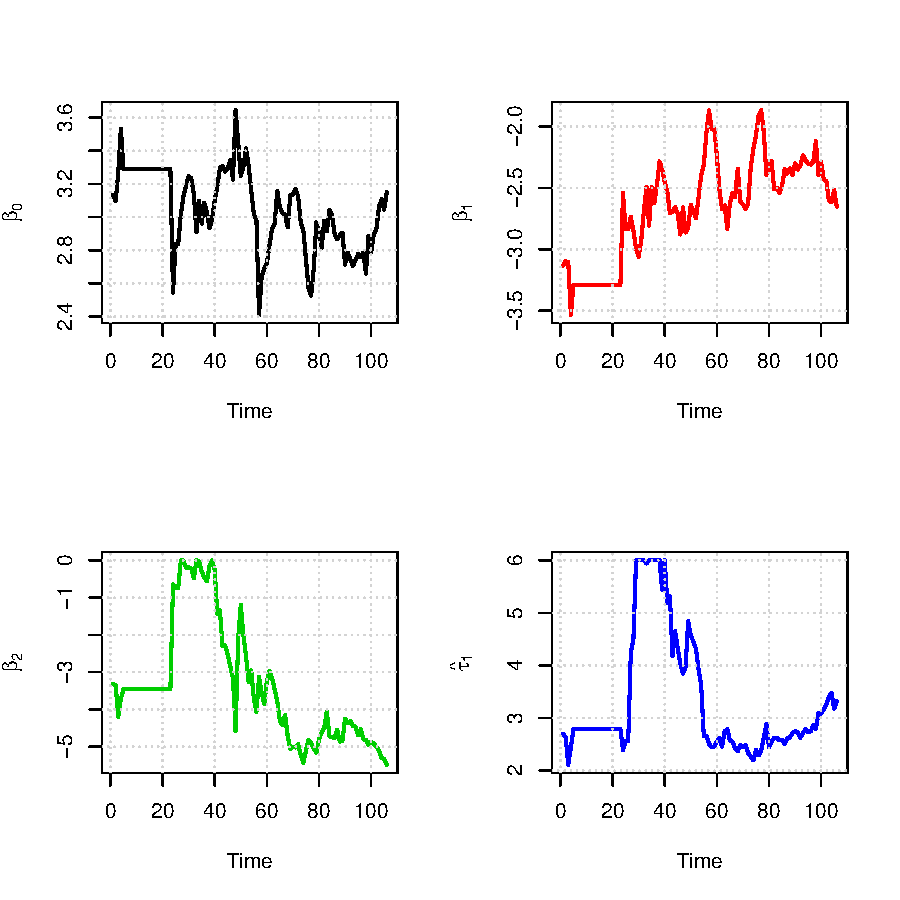
\includegraphics{Graduation_Paper-014}
\end{center}

\begin{center}
\begin{figure}[htbp]
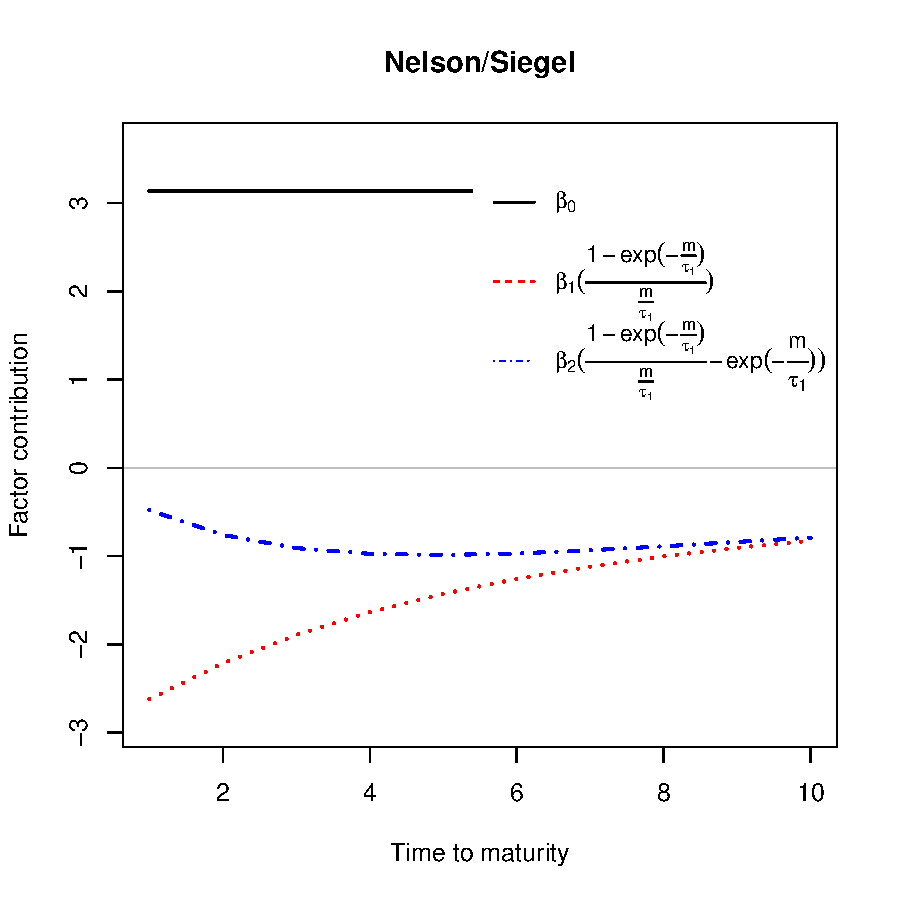
\includegraphics{Graduation_Paper-015}
\caption{Factor contribution, Japan data}
\end{figure}
\end{center}

\begin{Schunk}
\begin{Soutput}
---------------------------------------------------
Estimated Nelson/Siegel parameters:
---------------------------------------------------

Number of oberservations: 32 

[[1]]
     beta_0          beta_1            beta_2              tau_1       
 Min.   :4.138   Min.   :-4.6317   Min.   :-5.990951   Min.   :0.9051  
 1st Qu.:4.609   1st Qu.:-2.2995   1st Qu.:-3.909930   1st Qu.:1.3664  
 Median :4.866   Median :-1.0684   Median :-1.969124   Median :2.6834  
 Mean   :4.816   Mean   :-1.6972   Mean   :-2.232628   Mean   :2.9208  
 3rd Qu.:5.052   3rd Qu.:-0.6961   3rd Qu.:-0.374454   3rd Qu.:3.8958  
 Max.   :5.340   Max.   :-0.5281   Max.   :-0.000027   Max.   :6.0000  
\end{Soutput}
\end{Schunk}

\begin{center}
\begin{tabular}{|l||c|}\hline
                        & Goodness of fit \\ \hline
RMSE-yields (in \%)     & 0.0662619   \\ \hline
AABSE-yields (in \%)    & 0.0361092   \\ \hline
\end{tabular}
\end{center}


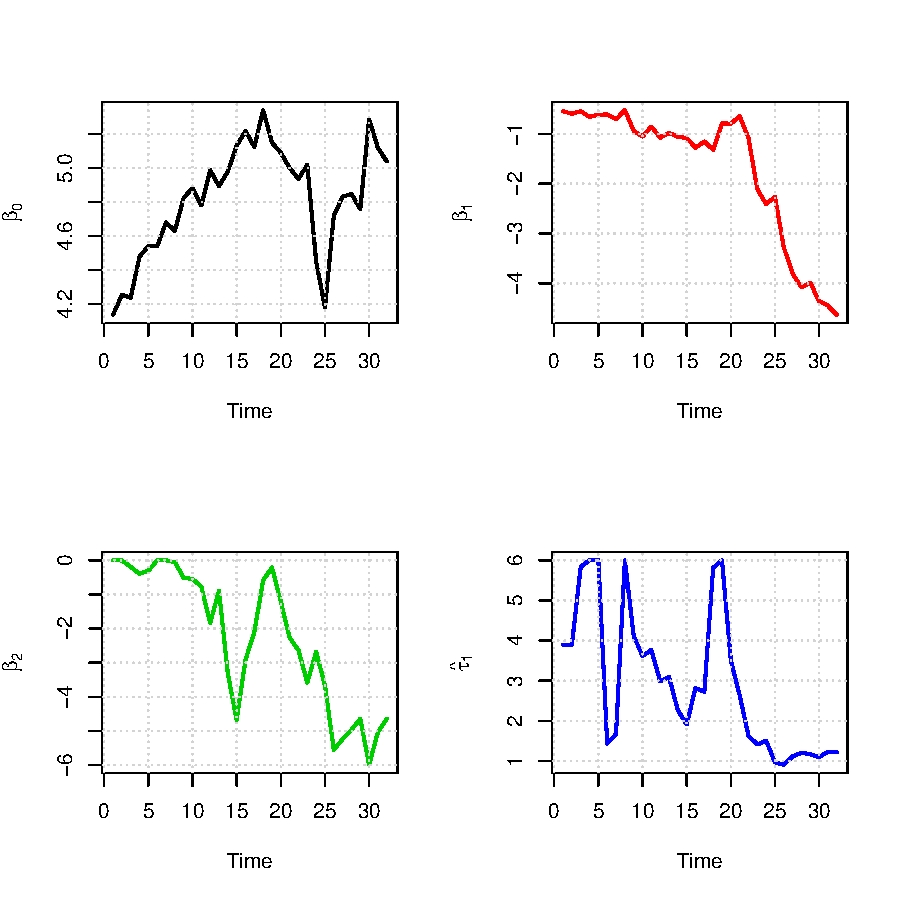
\includegraphics{Graduation_Paper-017}

\begin{center}
\begin{figure}[htbp]
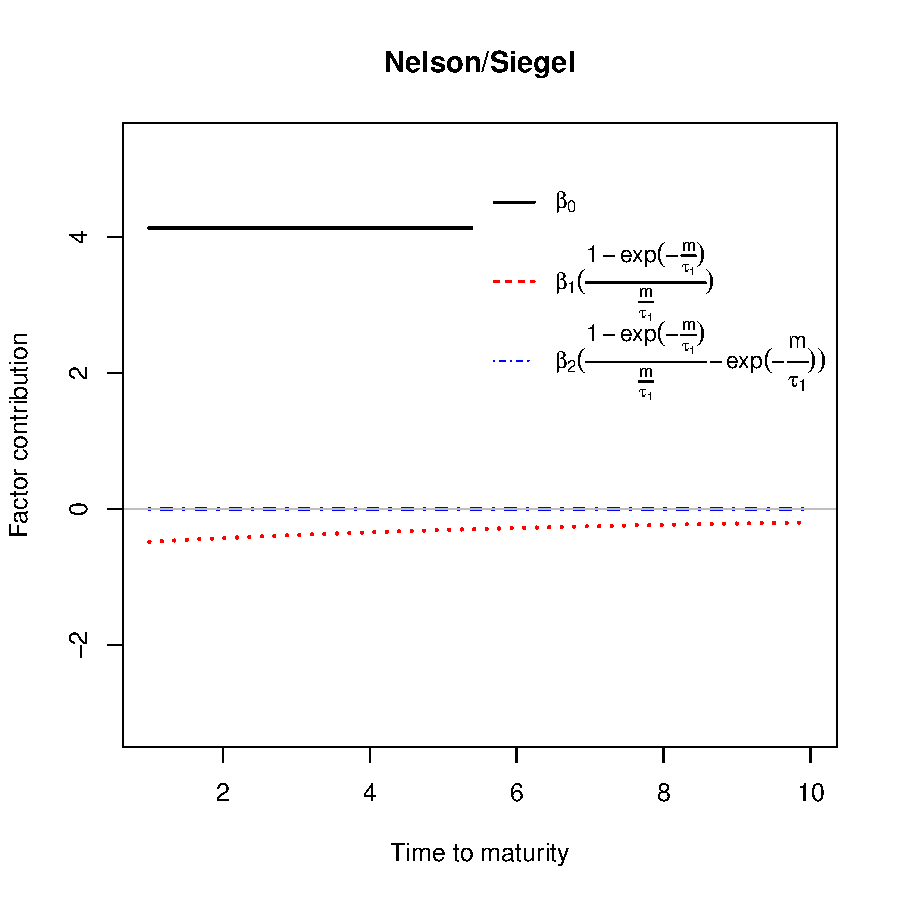
\includegraphics{Graduation_Paper-018}
\caption{Factor contribution, Euro data}
\end{figure}
\end{center}

It can be seen that if $\beta_1$ is negative, the forward curve will have a positive slope and other way round. The parameter $\beta_2$, indicates the magnitude and the direction of the hump and if it is positive, a hump will occur at $\lambda$. In case it is negative, a U-shaped value will occur at $\lambda$. So it can be concluded that parameter $\lambda$ could specify the position of the hump or U-shape on the entire curve. Consequently, Nelson and Siegel propose that with appropriate choices of weights for these three components, it's possible to generate a variety of yield curves based on forward rate curves with monotonic and humped shapes.

\subsection{Estimated parameter and actual yield curve}


\begin{center}
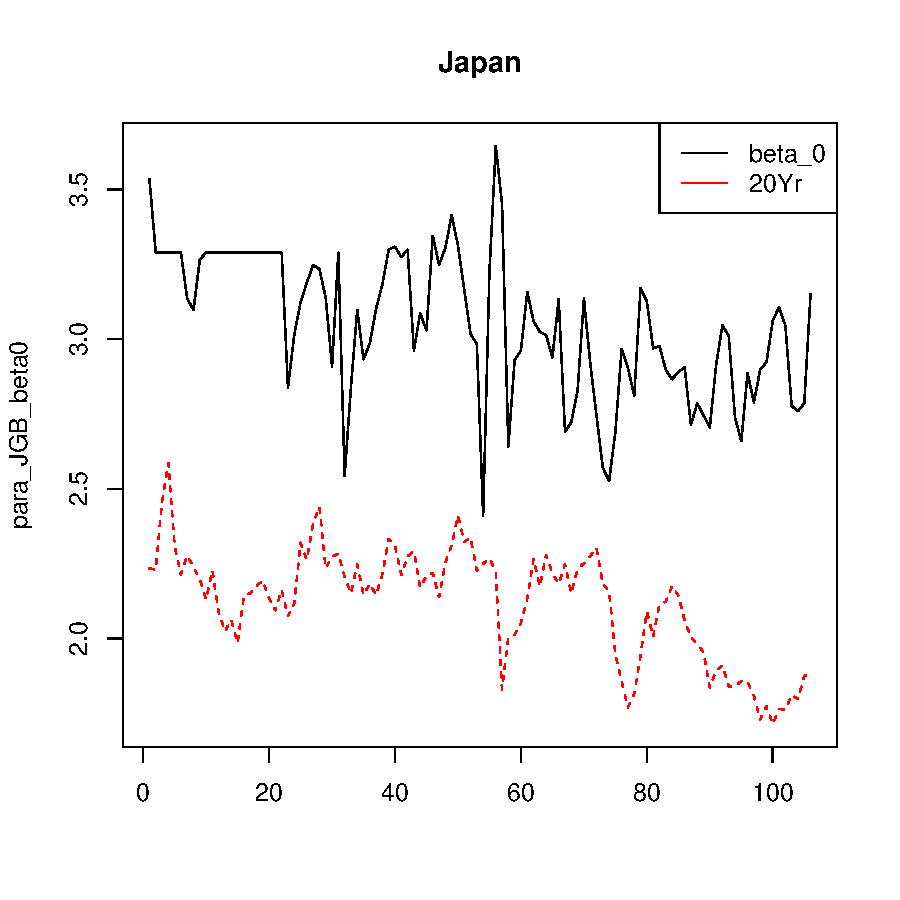
\includegraphics{Graduation_Paper-020}
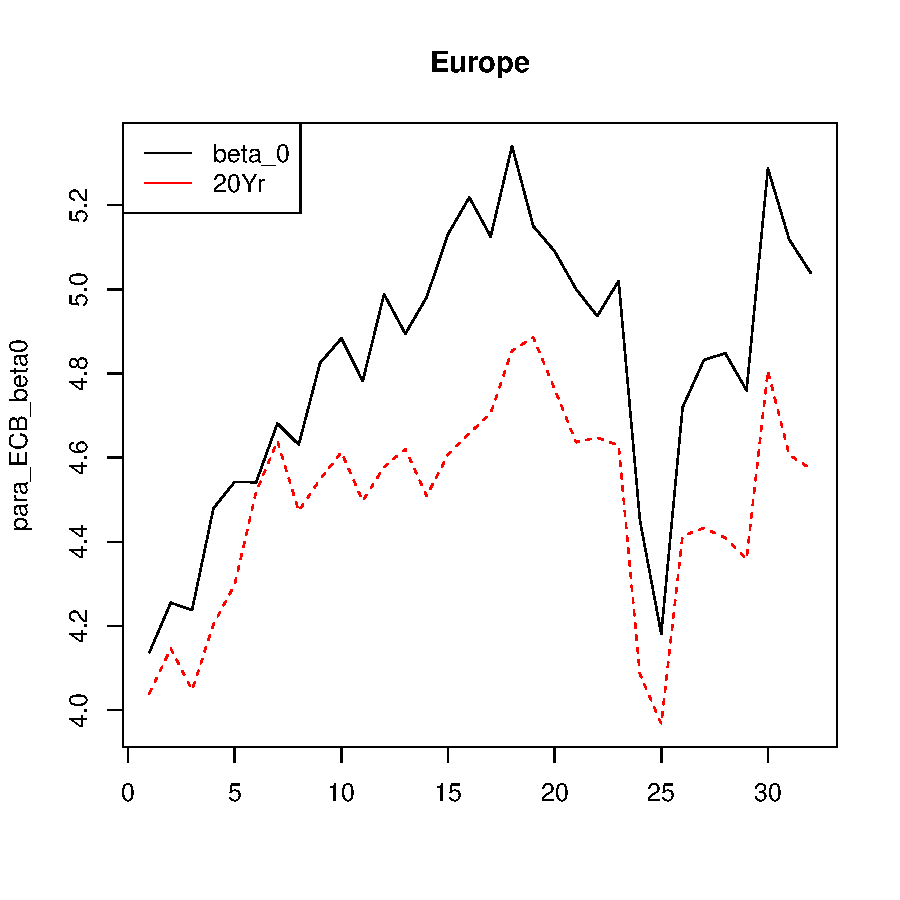
\includegraphics{Graduation_Paper-021}
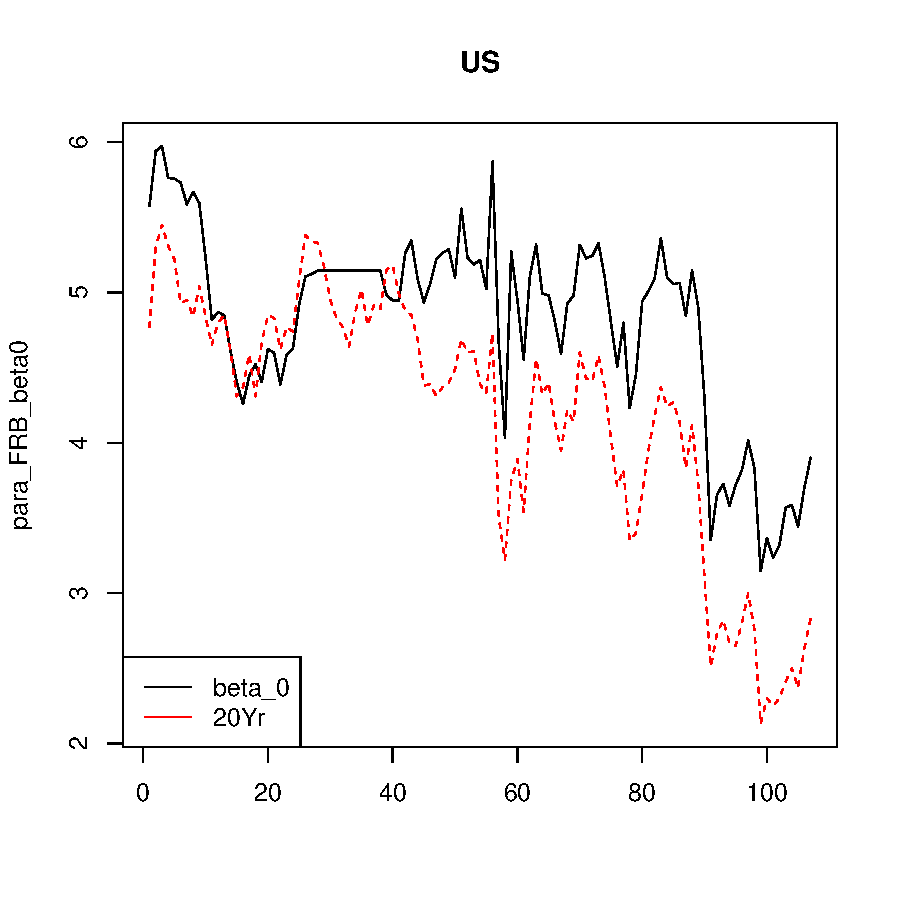
\includegraphics{Graduation_Paper-022}
\end{center}

In this 3 plots above, I compared the trending between $\beta_0$ with long term bonds, it is shown us that there exists correlation within them, we may be able to  establish AR(1) model for $\mathbf{\beta}$ to estimate yield curve, however, according to existing study, it does not work well.


\begin{center}
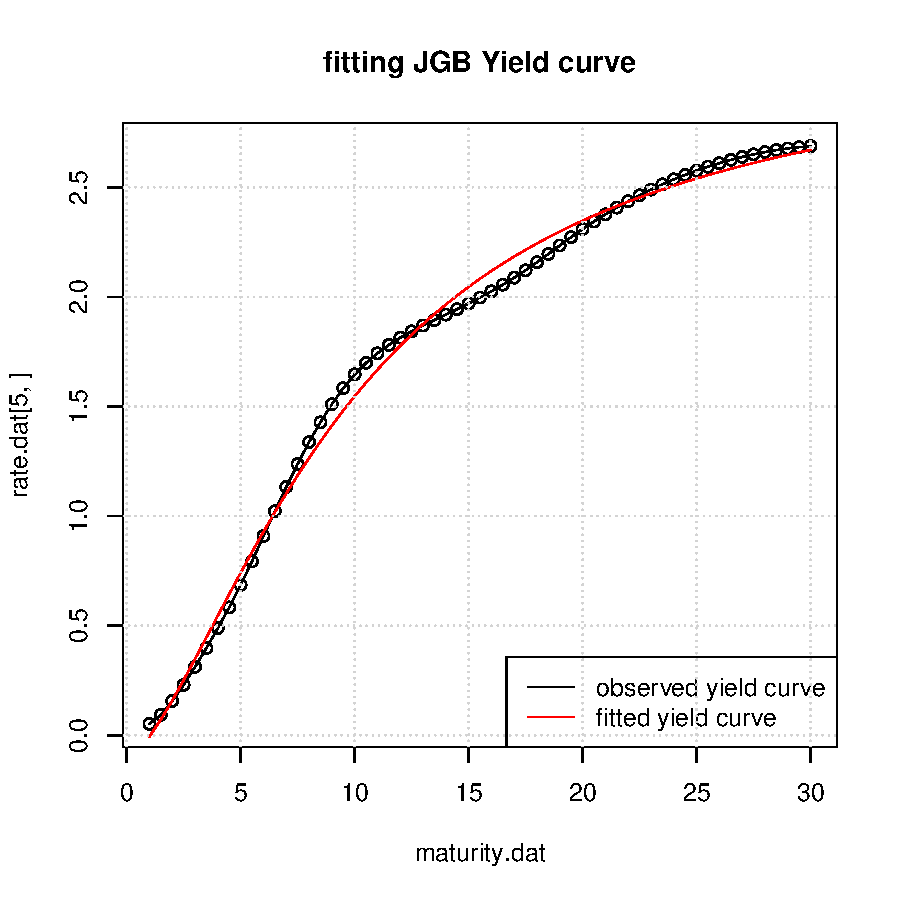
\includegraphics{Graduation_Paper-024}
\end{center}
I simulated historical yield curve of Japan at January 1st,2004, maturing to different term. It seems that the fitting for middle term yield curve is not as good as short term or long term.

\section{Principal Component Analysis(PCA) Approach}
\subsection{About PCA}
Principle Component Analysis(PCA) is a statistical method to aggregate multi-dimensional variables into lower number of dimensions and keep as much most important information as possible at the same time. Dissolution of time-series and multi-dimensional interest change data into non-correlated common components,as we already know, can explain the interest rate variances with lower number of variances, actually 3 principal components, that we call them as Parallel, Twist and Butterfly, which also was confirmed corresponding with those three interpreted as level, slope and curvature factors based on the factor loadings from the PCA (Diaz et al.2010).This principal component analysis also is a common method to analyse the bond valuation ability of alternative models on the first moment of interest rates (Olawale and Garwe, 2010; Huang and Chen, 2011. etc.).\\
R already has the function "prcomp(x)" for PCA, and we can take advantage of it.

\subsection{PCA of spot rate}
Analysis on JGB, US, Europe spot rate\\
Conditions\\
 \begin{itemize}
 \item\ Historical data of Japan,Unite State.
 
 \item\ Grid points:
 Maturing to  1Mo,3Mo,6Mo,1-30Yr
 \end{itemize}
\subsubsection{Results of US}



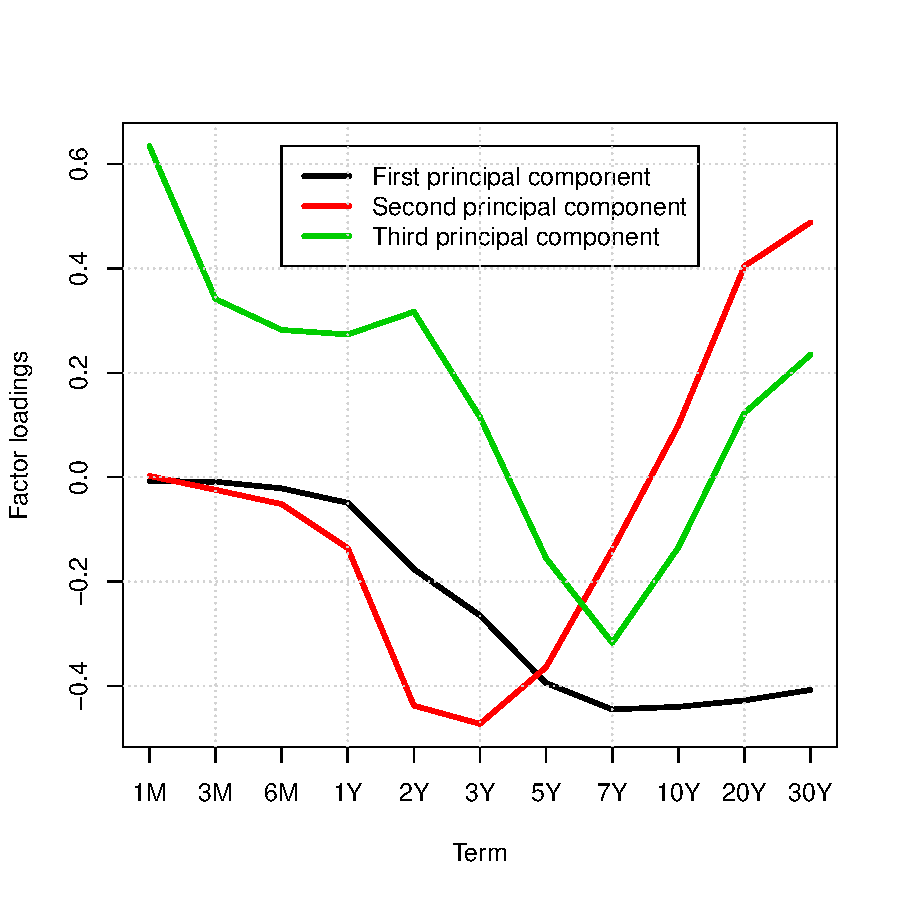
\includegraphics{Graduation_Paper-026}
\begin{center}
\begin{tabular}{|l||c||c||c|}\hline
                        & Comp.1 & Comp.2 & Comp.3 \\ \hline
Proportion of Variance  & 86.30\%& 7.59\% & 1.94\% \\ \hline
Cumulative Proportion   & 86.30\%&93.90\% & 95.80\%\\ \hline
\end{tabular}
\end{center}

 \subsubsection{Japan}

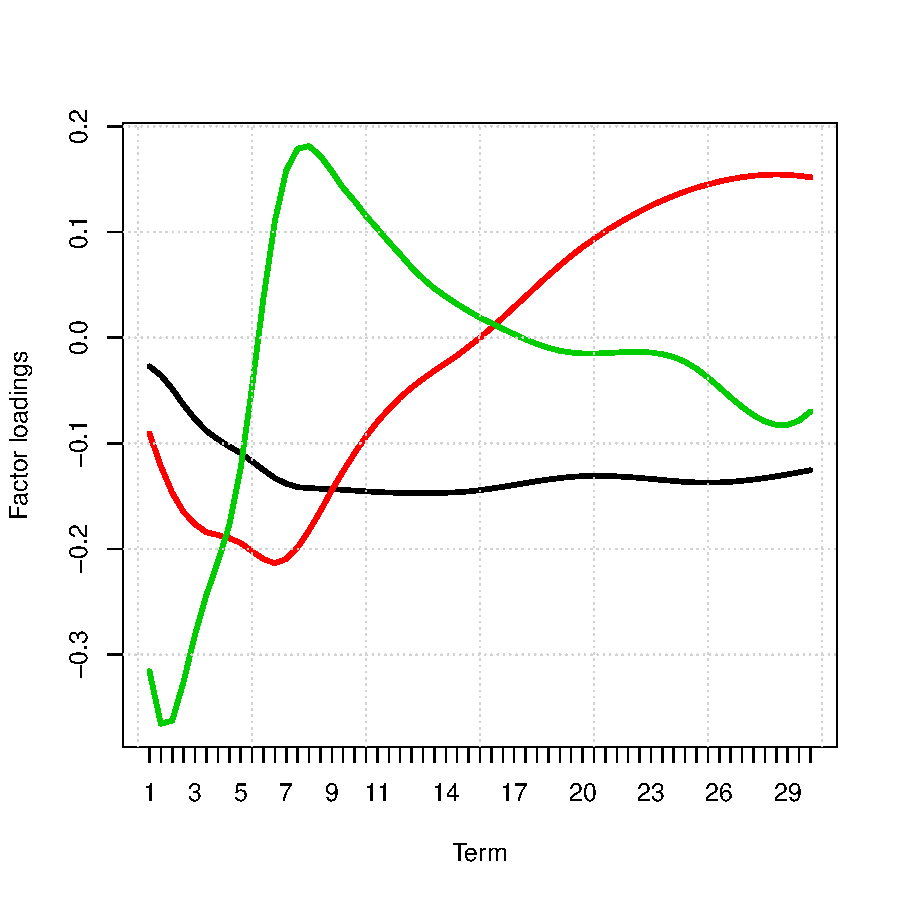
\includegraphics{Graduation_Paper-028}

\begin{center}
\begin{tabular}{|l||c||c||c|}\hline
                        & Comp.1 & Comp.2 & Comp.3 \\ \hline
Proportion of Variance  & 81.8\%& 14.0\% & 2.4\% \\ \hline
Cumulative Proportion   & 81.8\%&95.7\% & 98.1\%\\ \hline
\end{tabular}
\end{center}


 \subsubsection{Europe}

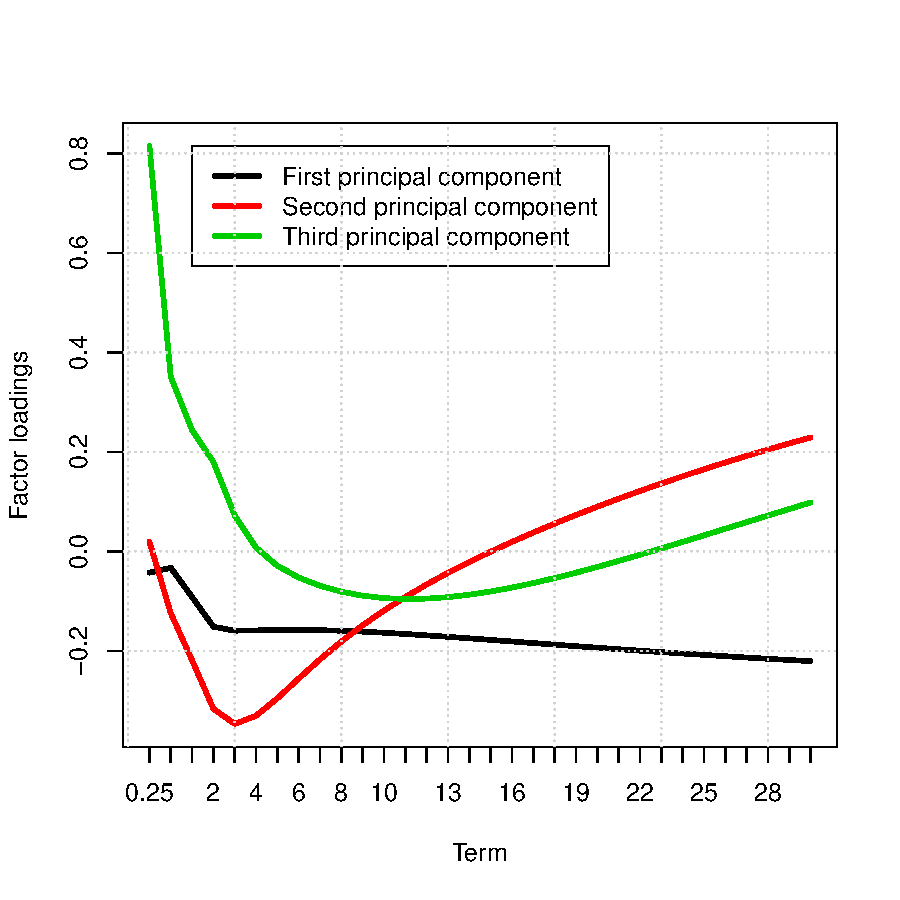
\includegraphics{Graduation_Paper-030}

\begin{center}
\begin{tabular}{|l||c||c||c|}\hline
                        & Comp.1 & Comp.2 & Comp.3 \\ \hline
Proportion of Variance  & 73.8\%& 16.0\% & 4.7\% \\ \hline
Cumulative Proportion   & 73.8\%& 89.8\% & 94.5\%\\ \hline
\end{tabular}
\end{center}

This study shows the proportion of the variance explained by each principal component and by principal components up to the order (the cumulative sum of the variance proportion). By analyzing historical volatility, we can see that that first three factors captured, in mean, about 98.1\% of the variation in the volatility time series in Japan market, compared to US market with 95.8\% and Europe market with 94.5\%, we can conclude that because Japan market is more flat than US and Europe in overall period, so the first three factors could explain a more high percentage of the variation than US and Europe.

\end{spacing}
\begin{thebibliography}{99}
\bibitem{Model}  Andrew J. G. Cairns(2004).
 \newblock \emph{Interest Rate Models\textendash An Introduction}.

\bibitem{} A.K.Tsui, J.X,wu and Z.Y.Zhang.
 \newblock Modelling the term structure of Japanese bond yields with the Nelson-Siegel model
 \newblock 20th International Congress on Modelling and Simulation, Adelaide, Australia, 1???6 December 2013
 
 \bibitem{} Charles R.Nelson, Andrew F.Siegel. 
 \newblock Parsimonious Modeling of Yield Curve.
 \newblock \textit{The Journal of Business, Vol.60, Issue 4}, 473-489.

\bibitem{} Damir filipovi\acute{c}, University of Munich.
 \newblock Interest rate models
 
 \bibitem{} David Bolder and David Streliski.
 \newblock Yield Curve Modelling at the Bank of Canada 
 \newblock http://laurent.jeanpaul.free.fr/Enseignement/bank_canada_yield_curve.pdf
 
 \bibitem{}Damiano Brigo(2007).
 \newblock "Interest Rate Models: Paradigm shifts in recent years".
 \newblock \url{http://ieor.columbia.edu/files/seasdepts/industrial-engineering-operations-research/pdf-files/Brigo_D.pdf}.
 
 \bibitem{} Enrico Schumann.
 \newblock Fitting the Nelson Siegel Svensson model with Differential Evolution.
 \newblock \url{http://cran.r-project.org/web/packages/NMOF/vignettes/DEnss.pdf}.
 
 \bibitem{} Francisco Jare\tilde{n}o and Marta Tolentino
 \newblock The US volatility term structure: A principal component analysis
 \newblock https://www.uclm.es/profesorado/fjareno/DOCS/Jare\%C3\%B1o\%20and\%20Tolentino\%20\%282012\%29.pdf
 
 \bibitem{} Jan Annaert, Anouk G.P Cales.  Estimating the Yield Curve Using the Nelson-Siegel Model

\bibitem{yield curve} Tomas Bjork and Bent Jesper Christensen(1997).
 \newblock interest rate dynamics and consistent forward rate curves,
 \newblock \url {http://swopec.hhs.se/hastef/papers/hastef0209.pdf}.

\bibitem{} Tea Poklepovic, Zdravka Aljinovic, Branka Marasovic.
 \newblock The Ability of Forecasting the Term Structure of Interest Rates Based on Nelson-Siegel and Svensson Model
 \newblock http://waset.org/publications/9997763/the-ability-of-forecasting-the-term-structure-of-interest-rates-based-on-nelson-siegel-and-svensson-model
 
\bibitem{} YU-Cheng Huang and Hantat Chen.
 \newblock The interaction among stock returns, the term structure of interest rates and economic activities: Evidence from Taiwan.
 \newblock http://www.academicjournals.org/article/article1380622303_Huang\%20and\%20Chen.pdf
  
 \end{thebibliography}

\end{document}
